\makeatletter
\def\input@path{{../../}}
\makeatother
\documentclass[../../main.tex]{subfiles}

\graphicspath{
	{../../img/}
	{../img/}
	{img/}
}

\begin{document}

\hrulefill

\bigskip

\begin{center}
{\it \textbf{Начиная со следующего раздела, лекции читал Кастрица О.~А.}} 
\end{center}

\hrulefill

\bigskip

\section{Семейство плоских кривых}

Пусть кривая задана параметрически:

 \begin{equation} \begin{cases}
 \label{lec18:1}
x=x(t),\\
y=y(t), \\
\alpha \le t \le \beta,
\end{cases}
\end{equation}

$k = y'_x = \frac{y'_t}{x'_t}$ \--- угловой коэффициент 
касательной к данной кривой.

Кривая может быть задана неявно:
\begin{equation}\label{lec18:2} F\left( x,y \right)  = 0, \end{equation}
при этом, если считать, что $y=y(x)$, то
\[ y'_x = - \frac{F'_x}{F'_y}.\]

Для кривой \eqref{lec18:1} предполагается, что
\[ \left( x' \left( t \right) \right)^2 + \left( y' \left( t \right) \right)^2 
\ne 0, \;  \forall t \in \left[ \alpha, \beta \right]. \]

Пусть, например, $x'\left( t_0 \right) \ne 0 $, тогда в окрестности точки 
$t_0$ 
функция $x\left( t \right) $ строго монотонна, а значит, существует обратная 
функция $t\left( x \right) $, и тогда:
\[ y = y \left( t \right) = y \left( t\left( x \right) \right), \]
т.~е. в $V \left( t_0 \right) $ эта кривая может быть задана уравнением
$y=y(x)$.
Если же $y'(t_0) \ne 0$, то соответствующим образом получаем, что в 
соответствующей окрестности $V \left( 
t_0 \right) $ она может быть задана уравнением $x=x\left( y \right) $.

Рассмотрим уравнение
\begin{equation} \label{lec18:3} F \left( x,y,c \right) = 0.  \end{equation}
Если зафиксировать значение $c$, то мы получаем некоторую кривую вида 
$\eqref{lec18:2}$. Т.~е. $\eqref{lec18:3}$ задает семейство плоских кривых, 
например:
\[ \left( x-c \right)^2 - y = 0. \]

\begin{center} 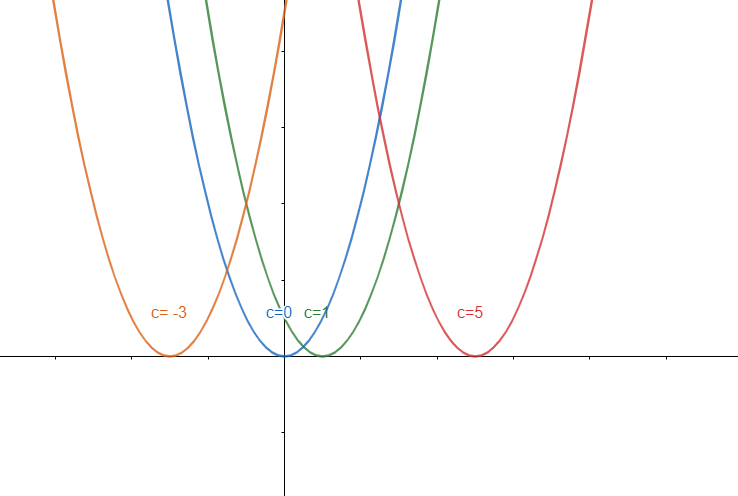
\includegraphics[scale=0.8]{first_family.png} \end{center}

Рассмотрим семейство 
\[ x^2 - y - c = 0 \]

\begin{center} 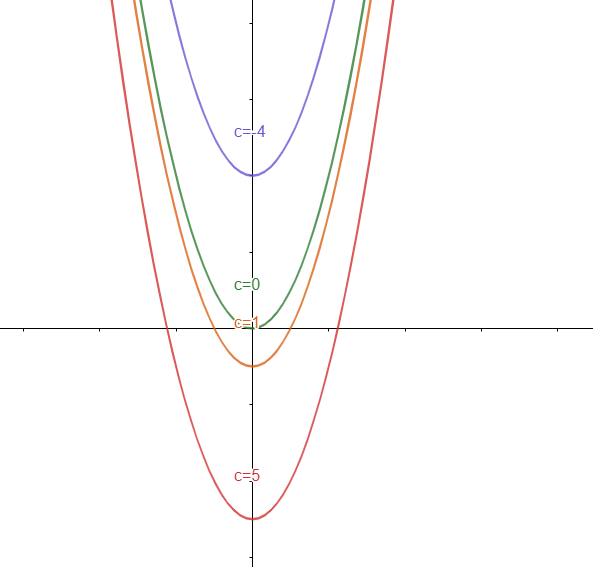
\includegraphics[scale=0.8]{second_family.png} \end{center}

Кривая $\lambda$ называется \emph{огибающей} семейство кривых 
$\eqref{lec18:3}$, если:

\begin{enumerate}
	\item В каждой точке $\lambda$ касается какой-либо кривой семейства 
	$\eqref{lec18:3}$.
	\item $\lambda$ касается всех кривых семейства $\eqref{lec18:3}$.
	\item $\lambda$ не имеет общей дуги ни с одной из кривых семейства 
	$\eqref{lec18:3}$.
\end{enumerate}

Возьмем какую-либо точку кривой $\lambda$. В этой точке $\lambda$ касается 
некоторой кривой из $\eqref{lec18:3}$, но эта кривая задается по $c$, 
т.~е. точке соответствует какое-либо $c = c_0$. Обратно, при любом $c$ мы 
получаем 
кривую из $\eqref{lec18:3}$ и соответствующую точку на огибающей $\lambda$.

Значит, $\lambda$ можно задать параметрическими уравнениями:
\[ \lambda: \begin{cases}
x=x\left( c \right), \\
y=y\left( c \right). 
\end{cases} \]

Касательная в точке касания имеет угловой коэффициент
$k = \frac{y' \left( c \right) }{ x' \left( c \right) }$.
С другой стороны, эта же касательная является касательной и для кривой 
семейства $\eqref{lec18:3}$, т.~е.
$k = - \frac{F'_x}{ F'_y}$.
Приравняв, получаем
\begin{equation}\label{lec18:4} F'_x\,x'(c) + F'_y\,y'(c) = 0.
\end{equation}

Точка $\left( x(c), y(c) \right) $ является точкой, 
соответствующей кривой семейства $\eqref{lec18:3}$ и, значит, $F(x(
c), y(c), c) = 0$.
Продифференцируем по $c$:
\begin{equation}\label{lec18:5} F'_x\, x'(c) + F'_y\,y'(c) + F'_c = 0. 
\end{equation}
Из $\eqref{lec18:4}$ и $\eqref{lec18:5}$ получаем, что $F'_c\left(x,y,c\right) 
= 0$. Добавляя \eqref{lec18:3}, получаем систему
\begin{equation}\label{lec18:6} \begin{cases}
F'_c\left(x,y,c\right) = 0,\\
F(x,y,c)  = 0.
\end{cases}  \end{equation}

Система $\eqref{lec18:6}$ \--- необходимое условие для огибающей.

Множество точек, удовлетворяющее системе $\eqref{lec18:6}$, называют 
\emph{дискриминантным множеством} или
\emph{дискриминантной кривой}.
Чтобы проверить, задают ли точки огибающую кривую, в общем случае нужны 
дополнительные исследования.

\begin{exmps}
\begin{enumerate}

\;

\item
$\left( x-c\right)^2 - y = 0$.

Составим уравнения вида $\eqref{lec18:6}$:
\[ \begin{cases}
-2\left( x-c\right)   = 0,\\
\left( x-c\right)^2 - y = 0
\end{cases} \text{откуда} \; y=0 \text{ \--- уравнение огибающей}. \]

\begin{center} 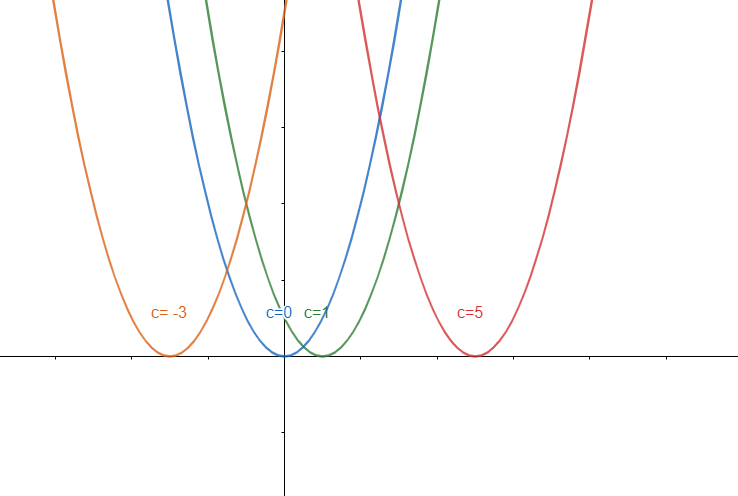
\includegraphics[scale=0.7]{first_family.png} \end{center}

Действительно, уравнение $y=0$ задает огибающую семейства $\left( x-c\right)^2 
- y = 0$.

\item
$x^2 - y - c = 0$.

\[ \begin{cases}
-1   = 0,\\
x^2 - y - c = 0.
\end{cases}  \]

Получаем противоречие $(-1 = 0)$, т.~е. дискриминантное множество 
пустое.

\item
$3\left( y - c\right)^2 = 2 \left( x-c \right)^3$.

Составим для этого семейства систему вида $\eqref{lec18:6}$:

\begin{gather*}
\begin{cases}
-6\left( y - c\right)  = -6 \left( x - c\right)^2,\\
3\left( y - c\right)^2 = 2 \left( x - c \right)^3
\end{cases} \implies
3\left( x-c\right)^4  = 2 \left( x-c\right)^3 \implies
x-c = \frac{2}{3}.
\end{gather*}
Подставляя, получаем:
\[ \begin{cases}
y-c  = \frac{4}{9}\\
x-c = \frac{2}{3}
\end{cases}  \implies
y - x = -\frac{2}{9}. \]

Но также существует и другое решение системы уравнений:  \[x-c = 0 \implies y 
- c = 0 \implies y = x. \]
Дискриминантное множество состоит из двух прямых, $y  = x - \frac{2}{9}$ и 
$y=x$. Рассмотрим полученные прямые:
\begin{center} 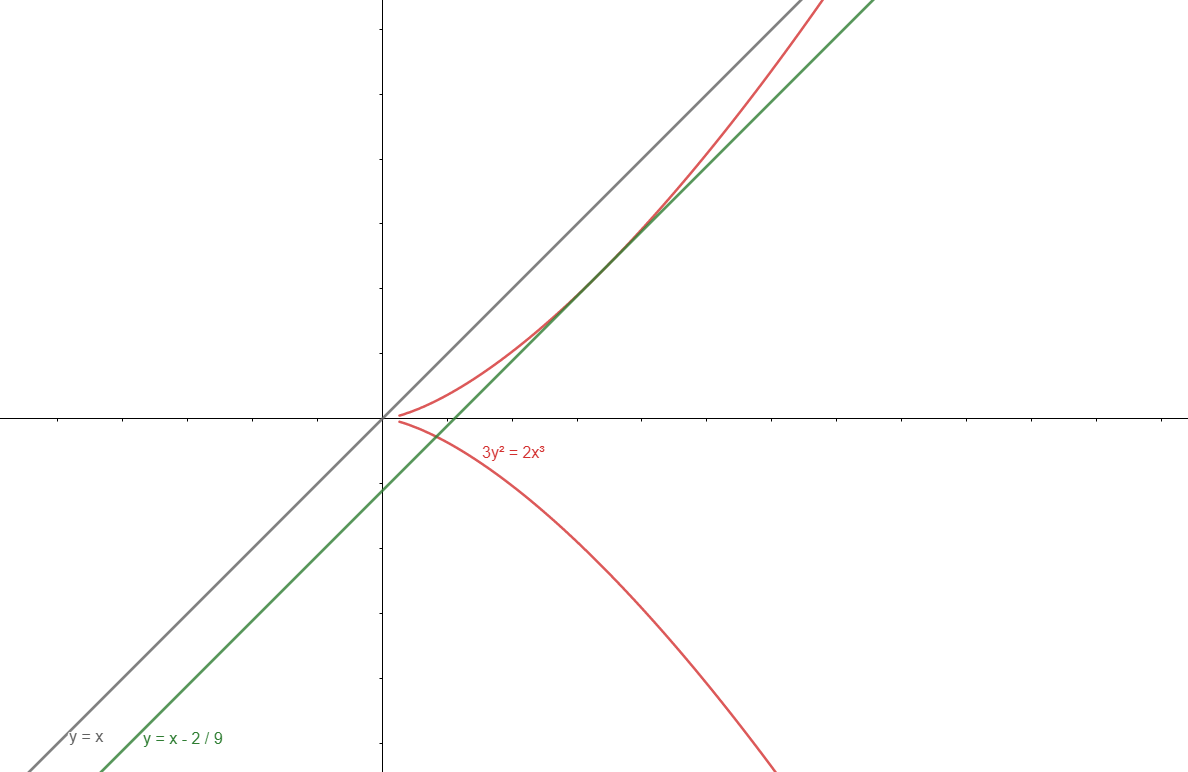
\includegraphics[scale=0.5]{hiperbola.png} \end{center}

При $c=0$ кривая $3y^2 = 2x^3$~--- полукубическая парабола. Меняя значение 
$c$, получаем сдвиг этой параболы.
Нетрудно видеть, что $y = x$ не является огибающей кривой, $y - x = 
-\frac{2}{9}$ является огибающей кривой.

\end{enumerate}
\end{exmps}

\section{Криволинейный интеграл первого рода (КрИ-1)}

Пусть задана спрямляемая кривая $\overbow{AB}$ и пусть $l$ \--- её длина. На 
ней задано направление из точки $A$ в точку $B$:

\begin{center} 
\begin{tikzpicture}[scale = 0.3]
		\node [style=none] (0) at (0, 0) {};
		\node [style=none] (1) at (5, 5) {};
		\node [style=none] (2) at (10, 10) {};
		\node [style=circle] (3) at (0, 0) {};
		\node [style=circle] (4) at (10, 10) {};
		\node [style=none] (13) at (1.35,0) {$A$};
		\node [style=none] (18) at (11.2499,10) {$B$};
		\draw [style=thin arrow, in=180, out=90] (0.center) to (1.center);
		\draw [bend right=45, looseness=0.75] (1.center) to (2.center);
\end{tikzpicture}
 
\end{center}

Пусть в точках этой кривой определена функция $f \left( x,y \right) $. 
Рассмотрим разбиение кривой $\overbow{AB}$ точками $A_k,\ k = \overline{0,n}$:
\begin{center}
\begin{tikzpicture}[scale = 0.5]
		\node [style=none] (0) at (0, 0) {};
		\node [style=none] (1) at (5, 5) {};
		\node [style=none] (2) at (10, 10) {};
		\node [style=circle] (3) at (0, 0) {};
		\node [style=circle] (4) at (10, 10) {};
		\node [style=circle] (5) at (0.675, 2.5) {};
		\node [style=circle] (6) at (3.25, 4.7) {};
		\node [style=circle] (7) at (6.625, 5.5) {};
		\node [style=circle] (8) at (8.975, 7.5) {};
		\node [style=rectangle] (9) at (0.15, 1.25) {};
		\node [style=rectangle] (10) at (1.8, 3.875) {};
		\node [style=rectangle] (11) at (7.85,6.35) {};
		\node [style=rectangle] (12) at (9.725, 8.75) {};
		\node [style=none] (13) at (1.75, 0) {$A=A_0$};
		\node [style=none] (14) at (2, 2.5) {$A_1$};
		\node [style=none] (15) at (4, 4) {$A_2$};
		\node [style=none] (16) at (8.25, 5) {$A_{n-2}$};
		\node [style=none] (17) at (10.5, 7.5) {$A_{n-1}$};
		\node [style=none] (18) at (11.75, 10) {$B = A_{n}$};
		\node [style=none] (19) at (1.5, 1.25) {$M_1$};
		\node [style=none] (22) at (3, 3.5) {$M_2$};
		\node [style=none] (23) at (9.25, 6) {$M_{n-1}$};
		\node [style=none] (24) at (11, 8.75) {$M_{n}$};
		\draw [style=thin arrow, in=180, out=90] (0.center) to (1.center);
		\draw [bend right=45, looseness=0.75] (1.center) to (2.center);
\end{tikzpicture}

\end{center}
Обозначим $\Delta s_k$ за длину дуги $\overbow{A_{k-1} A_k}$. $\delta = 
\max\limits_{k} \Delta s_k$ \--- диаметр разбиения.
На каждой дуге $\overbow{A_{k-1} A_k}$ возьмём точку $M_k \left( 
\widetilde{x_k}, \widetilde{y_k} \right) \in \overbow{A_{k-1} A_k}$ и 
построим сумму
\[ \sigma = \sum_{k=1}^{n} {f \left( \widetilde{x_k} , \widetilde{y_k} \right) 
\Delta s_k}.
\]
Точки $M_k$~--- промежуточные точки (как и для ОИ, 2И, 3И).

Предел
\[ \lim_{\delta \to 0} {\sigma} = \int\limits_{ \tiny{\overbow{AB}} }{f\left( 
x,y \right)ds } \]
называется \emph{криволинейным интегралом первого рода} (КрИ-1). Если этот 
предел существует и конечен, т.~е. равен некоторому числу, то 
говорят, что функция $f\left( x,y\right)$ интегрируема на кривой 
$\overbow{AB}$. Это будет тогда и только тогда, когда
\[ \forall \eps > 0 \quad \exists\,\delta_{\eps} \colon \forall \delta < 
\delta_{\eps} \; \left| \sigma - I \right| < \eps. \]

Мы будем предполагать, что функция $f$ ограничена на кривой, а если это не 
так, то конечный предел не будет существовать.
Необходимое условие интегрируемости \--- ограниченность функции на кривой.

\subsection{Геометрический смысл интеграла КрИ-1}

\begin{center} 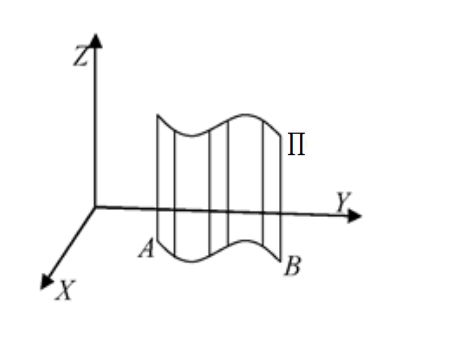
\includegraphics[scale=0.8]{lec18_pi.png} \end{center}

При довольно малом диаметре разбиения $f \left( \widetilde{x_k} , 
\widetilde{y_k} 
\right) \Delta s_k$ приближенно представляет площадь цилиндрической части 
поверхности, у которой, направляющая~--- $\overbow{AB}$, а образующая 
параллельна оси $Oz$.
Суммируя элементарные площади, получаем приближенную площадь поверхности 
$S_\Pi$.
Переходя к пределу при $\delta \to 0$, получаем
\[ \int\limits_{ \tiny{\overbow{AB}} }{f\left( x,y \right)ds} = \text{площадь} 
\; \Pi. \]

\subsection{Физический смысл интеграла КрИ-1}

На кривой $\overbow{AB}$ распределена масса с плотностью 
$\rho = \rho(x,y)$. Если выделить кусочек $\overbow{A_{k-1} A_k}$,
то при достаточно малом разбиении получаем $\Delta m_k \approx \rho \left( 
\widetilde{x_k} , \widetilde{y_k} \right) \Delta s_k$ (можем считать, что на 
нем плотность постоянна).
Суммируя элементарные массы и переходя к пределу, получаем:

\[ \int\limits_{ \tiny{\overbow{AB}} }{f\left( x,y \right)ds} = m = 
\text{масса кривой} \; \overbow{AB}. \]

\subsection{Вычисление КрИ-1}
\label{subsec:kri1-eval}

Пусть кривая $\overbow{AB}$ задана в естественной параметризации: 
\begin{equation}
\label{lec18:7}
 \begin{cases}
x=x(s),\\
y=y(s), \\
0 \le s \le l.
\end{cases}
\end{equation}

Тогда точке $A_k \left( x_k, y_k \right)$ соответствует $s_k$, которая 
порождает $\begin{cases}
x(s_k)\\
y(s_k) 
\end{cases}$.
Точке $M_k \left( \widetilde{x_k} , \widetilde{y_k} \right)$ соответствует 
$\widetilde{s_k}$, которая порождает $\begin{cases}
x(\widetilde{s_k})\\
y(\widetilde{s_k}) 
\end{cases}$. Тогда:

\begin{equation}
\label{lec18:8}
\sigma = \sum_{k=1}^{n} f\left( \widetilde{x_k} , \widetilde{y_k} \right) 
\Delta s_k = \sum_{k=1}^{n} f\left( x (  \widetilde{s_k} )  , y 
(  \widetilde{s_k}) \right)  \Delta s_k.
\end{equation}

Справа интегральная сумма для функции $f\left( x(s) ,y(s)  \right) $, 
построенная по разбиению отрезка $\left[ 0,l \right] $, с 
промежуточными точками $\widetilde{s_k}$~--- интегральная сумма для 
определенного 
интеграла
\[ \int\limits_{0}^{l} {f\left( x(s)  , y(s) \right) ds}.\]

Поэтому, переходя в $\eqref{lec18:8}$ к пределу, получаем:

\[\boxed{  \int\limits_{ \tiny{\overbow{AB}} }{f\left( x,y \right)ds} = 
\int\limits_{0}^{l} 
{f\left( x(s), y (s) 
\right) ds}. }\]

Пусть кривая $\overbow{AB}$ задана в произвольной параметризации:
\[  \begin{cases}
x=x(t),\\
y=y(t), \\
\alpha \le t \le \beta.
\end{cases} \]

Точке $A_k \left( x_k,y_k \right) $ соответствует значение параметра $t_k$, 
которое дает $\begin{cases}
x(t_k)\\
y(t_k) 
\end{cases}$.
Промежуточной точке $M_k \left( \widetilde{x_k} , \widetilde{y_k} \right) $ 
соответствует $\widetilde{t_k}$, что дает $\begin{cases}
x(\widetilde{t_k})\\
y(\widetilde{t_k}) 
\end{cases}$.

$\Delta s_k$ \--- длина дуги $\overbow{A_{k-1}, A_k}$, равна
\[ \int\limits_{t_{k-1}}^{t_k} {\sqrt{ \left( x' \left( t\right) \right)^2 + 
\left( 
y' \left( t\right) \right)^2  }} dt.
 \]
 
 В силу того, что мы рассматриваем гладкие кривые, т.~е. считаем, что $x(t), 
 y(t)$ непрерывные, по теореме о среднем получаем:
 
\[ \exists\: \overline{t_k} \in \left[ t_{k-1}, t_k \right] \colon \Delta s_k 
= \sqrt{ \left( x'( \overline{t_k}) 
\right)^2 + \left( y'( \overline{t_k}) \right)^2 }\: \Delta t_k.
\]

Т.~к. $\sqrt{ \left( x'( \overline{t_k}) 
\right)^2 + \left( y'( \overline{t_k}) \right)^2 }$ непрерывна на $\left[ 
\alpha, \beta \right] $ то по теореме 
Кантора она равномерно непрерывна на $\left[ \alpha, \beta \right]$, т.~е. ее 
значение при разных разбиениях мало изменится:

\[ \sqrt{ \left( x'( \overline{t_k}) 
\right)^2 + \left( y'( \overline{t_k}) \right)^2 } \Delta t_k = \left( \sqrt{ 
\left( x'( \widetilde{t_k}) 
\right)^2 + \left( y'( \widetilde{t_k}) \right)^2 } + \alpha_k\right) \Delta 
t_k, \]
где
\[ \alpha_k = \sqrt{ \left( x'( \overline{t_k}) 
\right)^2 + \left( y'( \overline{t_k}) \right)^2 } - \sqrt{ \left( x'( 
\widetilde{t_k}) 
\right)^2 + \left( y'( \widetilde{t_k}) \right)^2 }. \]
Поскольку 
$\sqrt{ \left( x'(t) \right)^2 + \left( y'(t) 
\right)^2  }$ непрерывна на $\left[ \alpha, \beta \right] $, а, значит,
равномерно непрерывна на этом отрезке, то $\alpha_k \appr{\delta \to 0} 0$. Но 
тогда

\[ \sigma = \sum_{k=1}^{n}{ f\left( \widetilde{x_k} , \widetilde{y_k} \right) 
\sqrt{ \left( x'( \widetilde{t_k}) 
\right)^2 + \left( y'( \widetilde{t_k}) \right)^2 }\:  \Delta t_k  } + 
\sum_{k=1}^{n}{ f\left( 
\widetilde{x_k} , \widetilde{y_k} \right) \alpha_k \Delta t_k}, \]
при этом $ \alpha_k \underset{\delta \rightarrow 0}
{\longrightarrow}  0$.
Переходя к пределу в интегральной сумме при $\delta \rightarrow 0$, получаем
\[ \boxed{\int\limits_{ \tiny{\overbow{AB}} }{f\left( x,y \right)ds} = 
\int\limits_{\alpha}^{\beta} {f \left( x\left( t\right) 
, y\left( t\right) \right) 
\sqrt{ \left( x'(t) \right)^2 + \left( y'(t) 
\right)^2 } dt}}. \]

Если кривая задана явным уравнением
\[ \overbow{AB} = \begin{cases} 
y = f\left( x \right), \\
\alpha \le x \le \beta,
\end{cases} \]
тогда ее легко задать параметрически:
\[ \begin{cases} 
x = t, \\
y = y \left( t \right), \\
\alpha \le t \le \beta.
\end{cases} \]
В этом случае
\[ \begin{cases} 
x = x, \\
y = y \left( x \right), \\
\alpha \le x \le \beta.
\end{cases} \]
Исходя из вышеизложенного, будем иметь:
\[ \boxed{\int\limits_{ \tiny{\overbow{AB}} }{f\left( x,y \right)ds} = 
\int_{\alpha}^{\beta} {f \left( x , y\left( x \right) \right) \sqrt{ 1 + 
\left( y'(x) \right)^2 } dx}.} \]

\begin{rem}
КрИ-1 не зависит от выбора направления по кривой $\overbow{AB}$. КрИ-1
обладает свойствами, общими для всех интегралов:
\begin{enumerate}
	\item Линейность:
	
	\[ \int\limits_{ \tiny{\overbow{AB}} }{\left(  \alpha f + \beta g \right)  \; 
	ds} = \alpha \int\limits_{ \tiny{\overbow{AB}} }{ f \; ds} + \beta 
	\int\limits_{ \tiny{\overbow{AB}} }{ g \; ds} \]
	
	Предполагается, что $f$ и $g$ интегрируемы, т.~е. все интегралы существуют.
	
	\item Аддитивность:
	
	\[ C \in \overbow{AB} \implies
	\int\limits_{ \tiny{\overbow{AB}} }{f  \; ds} = \int\limits_{ 
	\tiny{\overbow{AC}} }{f  \; ds} + \int\limits_{ \tiny{\overbow{CB}} }{f  \; 
	ds}. \]
	Предполагается, что $f$ интегрируема.
	
	\item Монотонность:
	
	Если для интегрируемых на $\overbow{AB}$ функций $f$ и $g$ выполняется $f \le 
	g$, то:
	\[ \int\limits_{ \tiny{\overbow{AB}} }{f  \; ds} \le \int\limits_{ 
	\tiny{\overbow{AB}} }{g  \; ds}.\]
	
	\item Основная оценка:
	
	Пусть для интегрируемой $f$ на $\overbow{AB}$ выполняется
	\[ m \le f ( x,y ) \le M ,\ \forall \left( x,y 
	\right) \in \overbow{AB}.\]
	Тогда, если обозначить за $l$ длину $\overbow{AB}$, выполняется
	\[ ml \le \int\limits_{ \tiny{\overbow{AB}} }{f  \; ds} \le Ml. \]
	
	\item Теорема о среднем:
	
	Если $f$ непрерывна на $\overbow{AB}$, то
	
	\[ \exists \left(x_0, y_0 \right) \in 
	\overbow{AB}\text{, такая, что }\int\limits_{ \tiny{\overbow{AB}} }{f  \; ds} 
	= f\left( x_0, y_0 \right) l.
	\]
	
\end{enumerate}
	
\end{rem}

Эти свойства вытекают из свойств определенных интегралов, к которым сводится 
\mbox{КрИ-1}.

\begin{exmp}
	Вычислить
	$\displaystyle \int\limits_{ \tiny{\overbow{AB}} }{\left( x^2 + xy \right) 
	ds}$, 
	где $\overbow{AB}$ \--- отрезок $A\left( 0,0 \right)$, 
	$B\left( 1,2 \right)$.
	
	\[ \int\limits_{ \tiny{\overbow{AB}} }{\left( x^2 + xy \right) ds} = \left[ 
	\overbow{AB} = \begin{cases} y = 2x \\ 0 \le x \le 1 \end{cases}\right] = 
	\int_{0}^{1} \left( x^2 + 2x^2 \right) \sqrt{1+4} \; dx =  \sqrt{5}. \]
\end{exmp}

\end{document}
